\documentclass[12pt]{gshs_beamer_class}
% beamer ver2.0의 수정 사항
% 1. 기존 붉은색 이외에 녹색과 푸른색의 beamer도 제작 가능함 (색 변조한 학교 아이콘 ./logo 폴더에 탑재)
% 2. 수식 및 소스 코드 폰트 변경 부분 추가
% 3. 타이틀 페이지의 학교 아이콘을 벡터 이미지로 수정 및 크기 조정

%%%%%%%%%% *** Packages %%%%%%%%%%
%%%% 1) Following packages are included in the *.cls file:
%\usepackage{ifthen}
%\usepackage{xcolor}
%\usepackage{amssymb,amsmath,graphicx}
%\usepackage{etoolbox}
%\usepackage[hangul]{kotex}
%\usepackage{tikz}
%\usepackage{listings}

%%%% 2) Additional packages
\usepackage{framed}
\usepackage{array}
\usepackage{siunitx}
\usepackage{lipsum}


%%%%%%%%%% *** Beamer Style Settings %%%%%%%%%%
%%%% 1) Theme Color
\themecolor{red} %red, green, blue

%%%% 2) Equations Font Setter
% rm: classical LaTeX math font
% sf: cleaner font
\equationfont{rm} %rm, sf

%%%% 3) Listing (Source Code) Font Setter
% If you want to use typewriter font in listing environments, please delete the command below.
\usepackage{inconsolata}

%%%% 4) ToC Auto Producer
% ToC frame is added at the beginning of every section.
% If you want a title at ToC frames, please write the frametitle after 'begin frame.'
\AtBeginSection[]
{
\begin{frame}{}
	\tableofcontents[currentsection]
\end{frame}
}

%%%% 5) Line Strecth Setter
\renewcommand{\baselinestretch}{1.1}



%%%%%%%%%% *** The Title %%%%%%%%%%
\title[]{발표 주제를 입력하세요\\\small{Your Presentation Topic}}
\subtitle[]{선형대수학 (2020-2)}
\author[]{19XXX OOO}
\institute[]{과학영재학교 경기과학고등학교}
\date[]{\today}



%%%%%%%%%% *** The Body %%%%%%%%%%
\begin{document} \small

\begin{frame}[plain] %title page
	\titlepage
\end{frame}

\setbeamertemplate{sidebar left}[sidebar theme] %sidebar


\begin{frame}[t]{Introduction}
	매우 유익한 글이므로 숨은 뜻을 해석해보자.\\
	\lipsum[1] Guman araboza.
\end{frame}


\section{Drawings}
\begin{frame}[t]{Separated Balls}
	\centering
	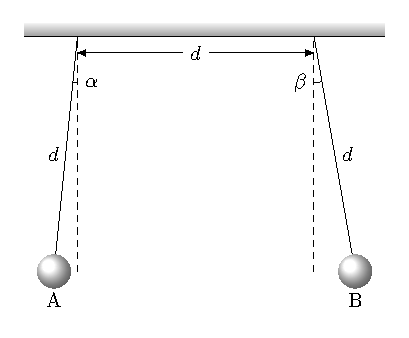
\includegraphics[width=0.7\textwidth]{./figures/practice.pdf} \\
	
	\begin{minipage}{0.45\textwidth}
		\centering
		$\rm A$ moves toward left.
	\end{minipage}
	\begin{minipage}{0.45\textwidth}
		\centering
		$\rm B$ moves toward right.
	\end{minipage}
\end{frame}

\begin{frame}[t]{Plate Falling}
	\centering
	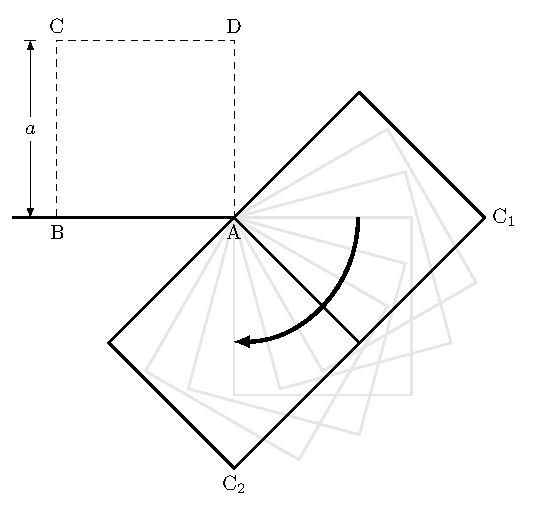
\includegraphics[width=0.7\textwidth]{./figures/plate.pdf}
\end{frame}


\section{Additional Functions}

\subsection{Blocks}

\begin{frame}[t]{Theorem Block}
	Block 환경을 적절히 쓰면 멋진 beamer를 만들 수 있다.
	\begin{block}{Cramer's Rule}
		Let $A$ be an \underline{invertible} \underline{$n \times n$} matrix, and let $\mathbf{b}$ be a vector in $\mathbb{R}^n$. Then the unique solution $ \mathbf{x} $ of the system $A\mathbf{x} = \mathbf{b}$ is given by
		\begin{equation*}
			x_i = \frac{\mathrm{det} ( A_i (\mathbf{b}))}{\mathrm{det} A}  \; \; \; \; \; (i = 1, ~ 2, ~\cdots , ~n)
		\end{equation*}
	\end{block}
	\vspace{15pt}
	$A$는 invertible하므로,
	\begin{itemize}
		\item $A\mathbf{x} = \mathbf{b}$는 유일한 해를 가짐.
		\item $ \mathrm{det} A \neq 0 $
	\end{itemize}
\end{frame}

\begin{frame}[t]{Summary Block}
\begin{block}{Binding-Change Mechanism}
	\begin{enumerate}\scriptsize
		\item F$_O$ 구역을 통해 H$^+$가 움직인다. (회전 동력 공급)
		\item 회전 구역인 c, $\gamma$, $\epsilon$가 회전한다.
		\item F$_1$ 구역의 $\beta$ 조각이 구조가 바뀌면서 ADP + P$_i$를 이용하여 ATP를 합성한 후 뒤이어 ATP를 방출한다.
	\end{enumerate}
\end{block}
\end{frame}

\begin{frame}[t, fragile]{Listing Block}
	sine 함수가 꺾인 선처럼 보인다면? Sample의 수를 조정한다.\\
	\vspace{5pt}
	\centering
	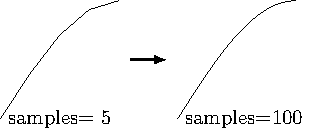
\includegraphics[width=0.5\linewidth]{./figures/samplenumbers.pdf}
	
	\begin{block}{}
		\begin{lstlisting}
\draw[domain=0:5, samples=100, variable=\x] 
	plot({\x}, {3 + sin(90*\x)});
		\end{lstlisting}
	\end{block}
\end{frame}

\subsection{Animations}
\begin{frame}[t]{Animations}
	정적인 pdf에서 현란한 애니메이션을 구현하기는 어렵다. ppt로 치면 `나타내기' 정도의 간단한 애니메이션을 넣을 수는 있다.
	
	\begin{itemize} \pause
		\item \textbackslash pause 명령을 쓰면 쓴 곳마다 프레임이 끊긴다. \pause
		\item \textbackslash onslide는 복잡한 순서도 구현해준다. \pause
		\item Ti\textit{k}Z의 \textbackslash foreach 반복문이랑 결합하면 그림 요소에도 애니메이션을 넣을 수 있다.	
	\end{itemize}

\end{frame}

\end{document}
